\documentclass[slidestop]{beamer}

\usepackage[english]{babel}

\title{Diagnostic Variant Database:\\ design and implementation}
\providecommand{\myConference}{BioAssist programmers meeting}
\providecommand{\myDate}{Friday, 17 August 2012}
\author{Martijn Vermaat}
\providecommand{\myGroup}{}
\providecommand{\myDepartment}{Department of Human Genetics}
\providecommand{\myCenter}{Center for Human and Clinical Genetics}
\providecommand{\lastCenterLogo}{
%  \raisebox{-0.1cm}{
%    
\includegraphics[height = 1cm]{lgtc_logo}
%  }
}
\providecommand{\lastRightLogo}{
  
\includegraphics[height = 0.7cm]{nbic_logo}
  %\includegraphics[height = 0.8cm]{nwo_logo_en}
}

\usetheme{lumc}

\begin{document}

% This disables the \pause command, handy in the editing phase.
%\renewcommand{\pause}{}

% Make the title page.
\bodytemplate

\frame{
  \frametitle{Diagnostic Variant Database}
  \tableofcontents
}

\section{Introduction}

\begin{frame}
  \frametitle{Background}
  NGS produces a large number of genomic variants
  \begin{itemize}
    \item Valuable to medical research
    \item Several groups have their own ad-hoc database
    \item Not easily coupled (technically and politically)
  \end{itemize}
  \vspace{1cm}
  \pause
  Collaboration needed
  \begin{itemize}
    \item Central human genomic variant database
    \item LUMC, UMCU, UMCN, UMCG
    \item Only accessible to collaborators
    \item Using is sharing
    \item Coordinated by NBIC Bio-Assist
  \end{itemize}
\end{frame}

\section{Data model}

\begin{frame}[fragile]
  {\bf \it Variants}
  \begin{itemize}
    \item Genomic location
    \item Reference sequence
    \item Variant sequence
  \end{itemize}
  \vspace{0.8cm}
  {\bf \it Covered regions}
  \begin{itemize}
    \item Genomic start and end location
  \end{itemize}
  \vspace{0.2cm}
  \begin{center}
    \only<1,2>{\visible<2>{
\includegraphics[width=0.8\textwidth]{coverage1}}}\only<3>{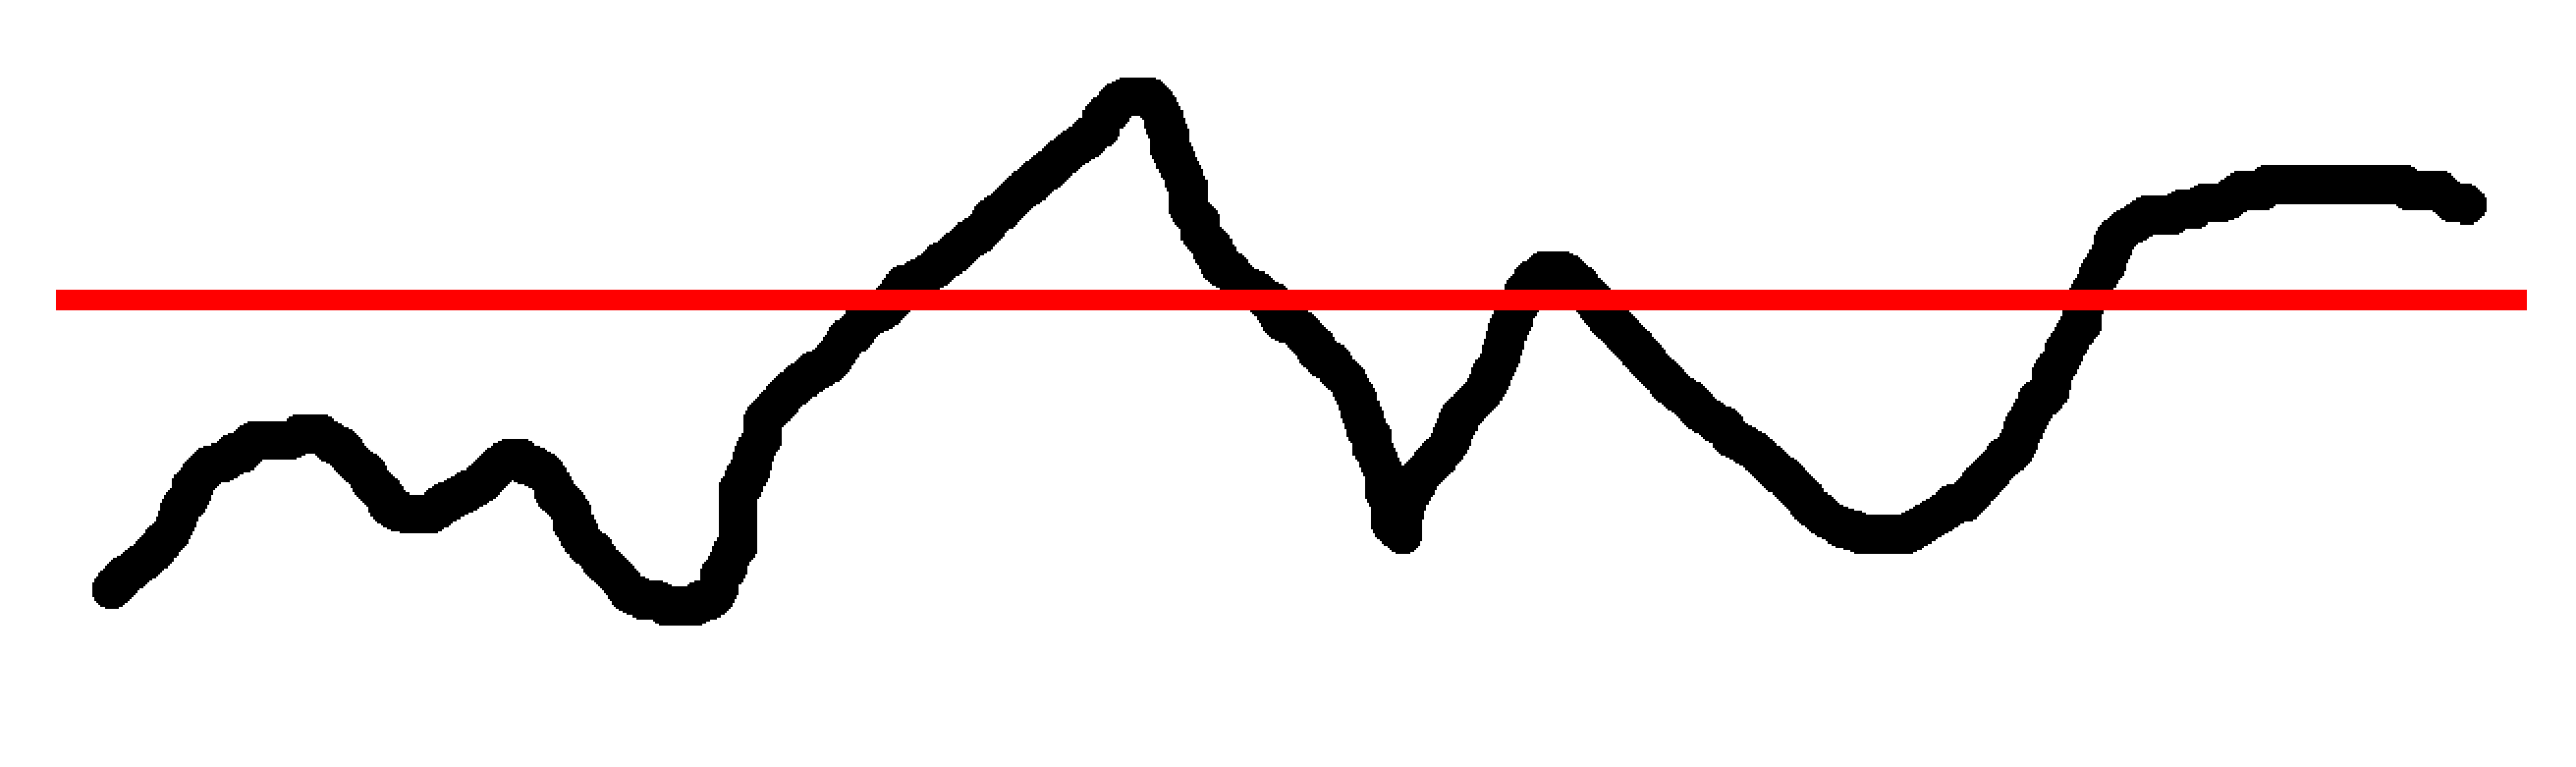
\includegraphics[width=0.8\textwidth]{coverage2}}\only<4>{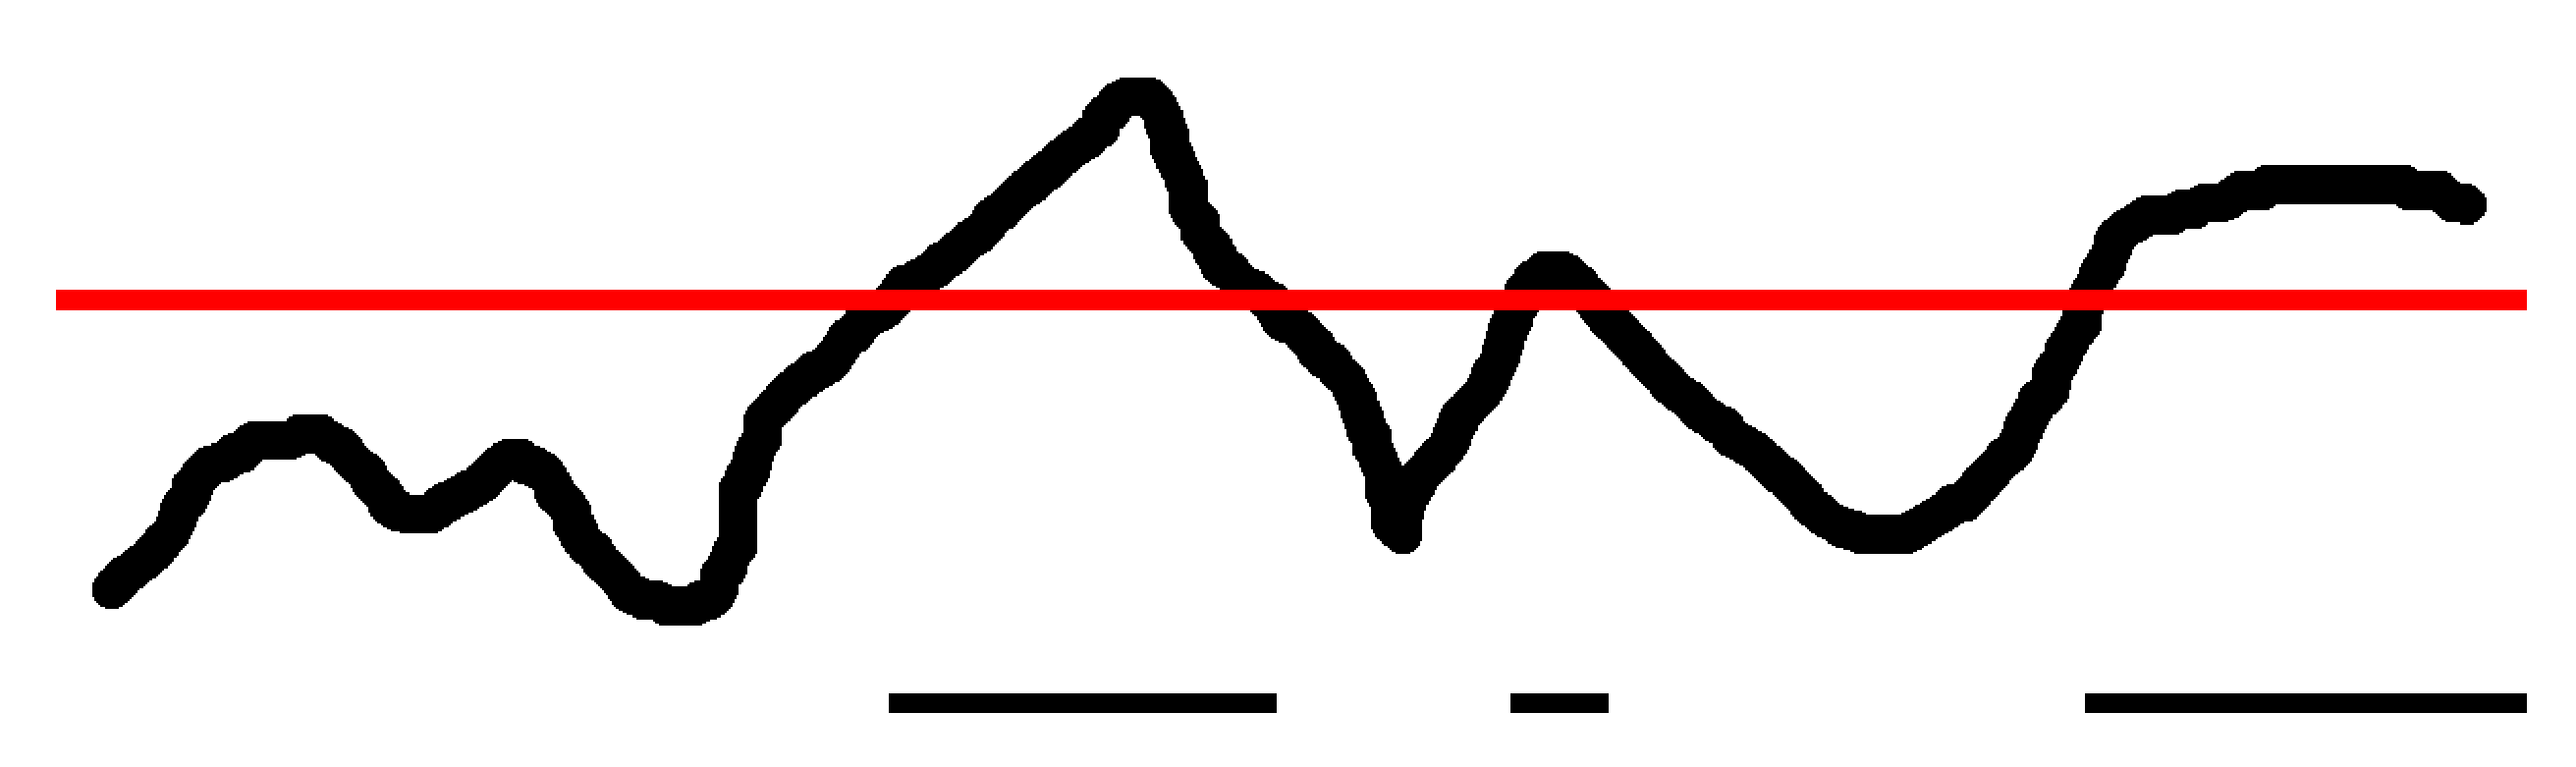
\includegraphics[width=0.8\textwidth]{coverage3}}
  \end{center}
\end{frame}

\begin{frame}
  \frametitle{Variant frequency example}
  \begin{center}
    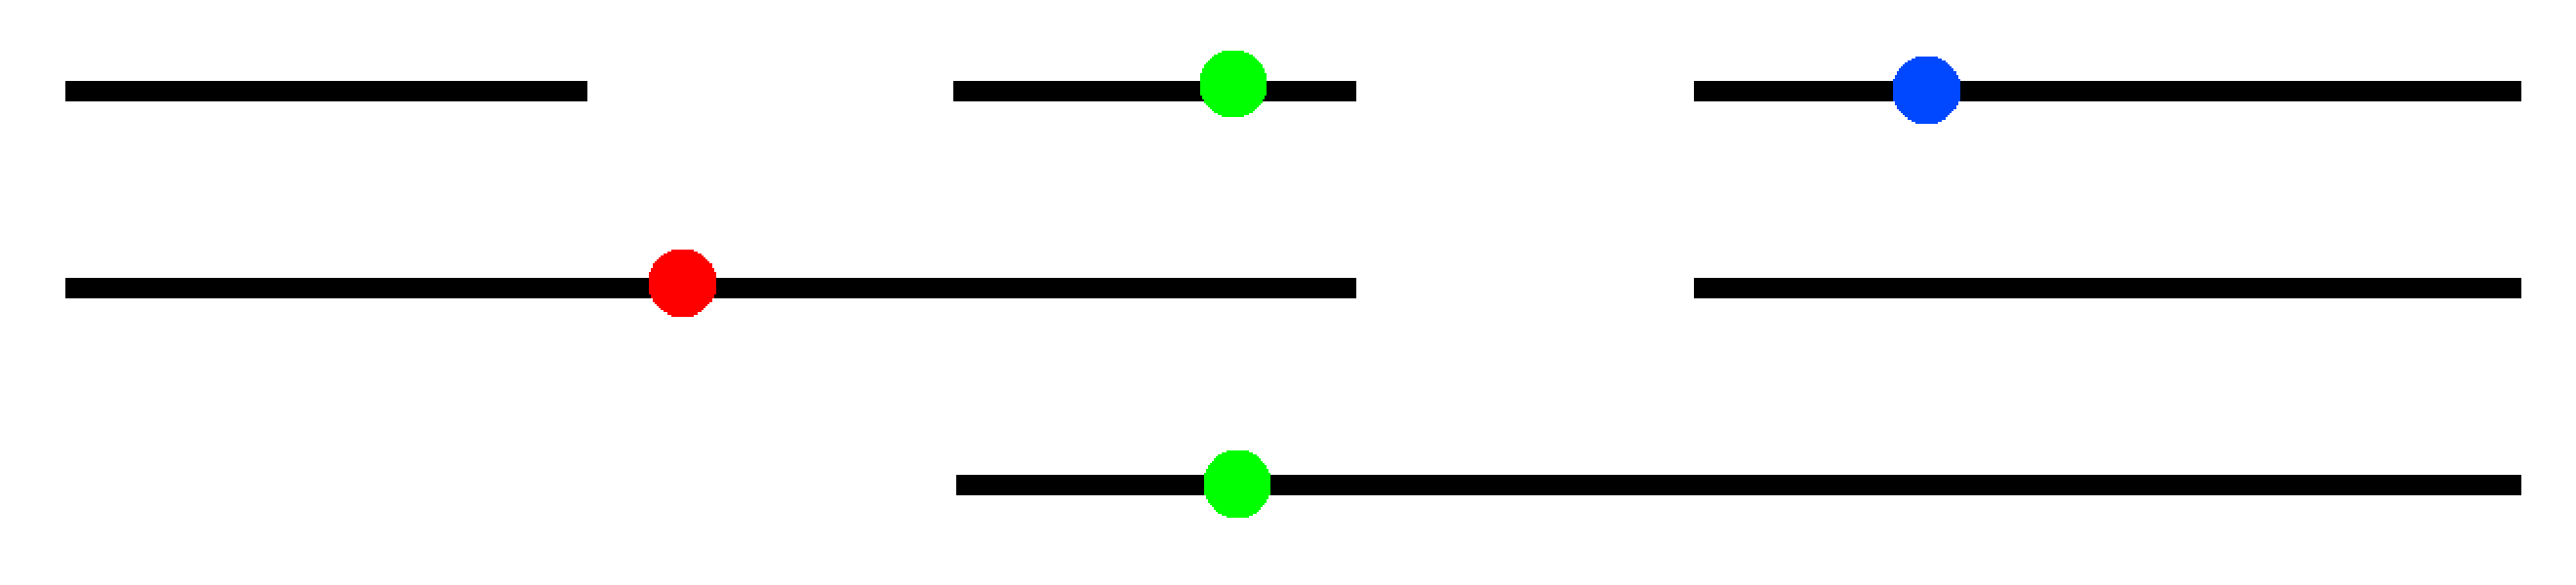
\includegraphics[width=\textwidth]{frequencies}
  \end{center}
\end{frame}

\begin{frame}
  \begin{center}
    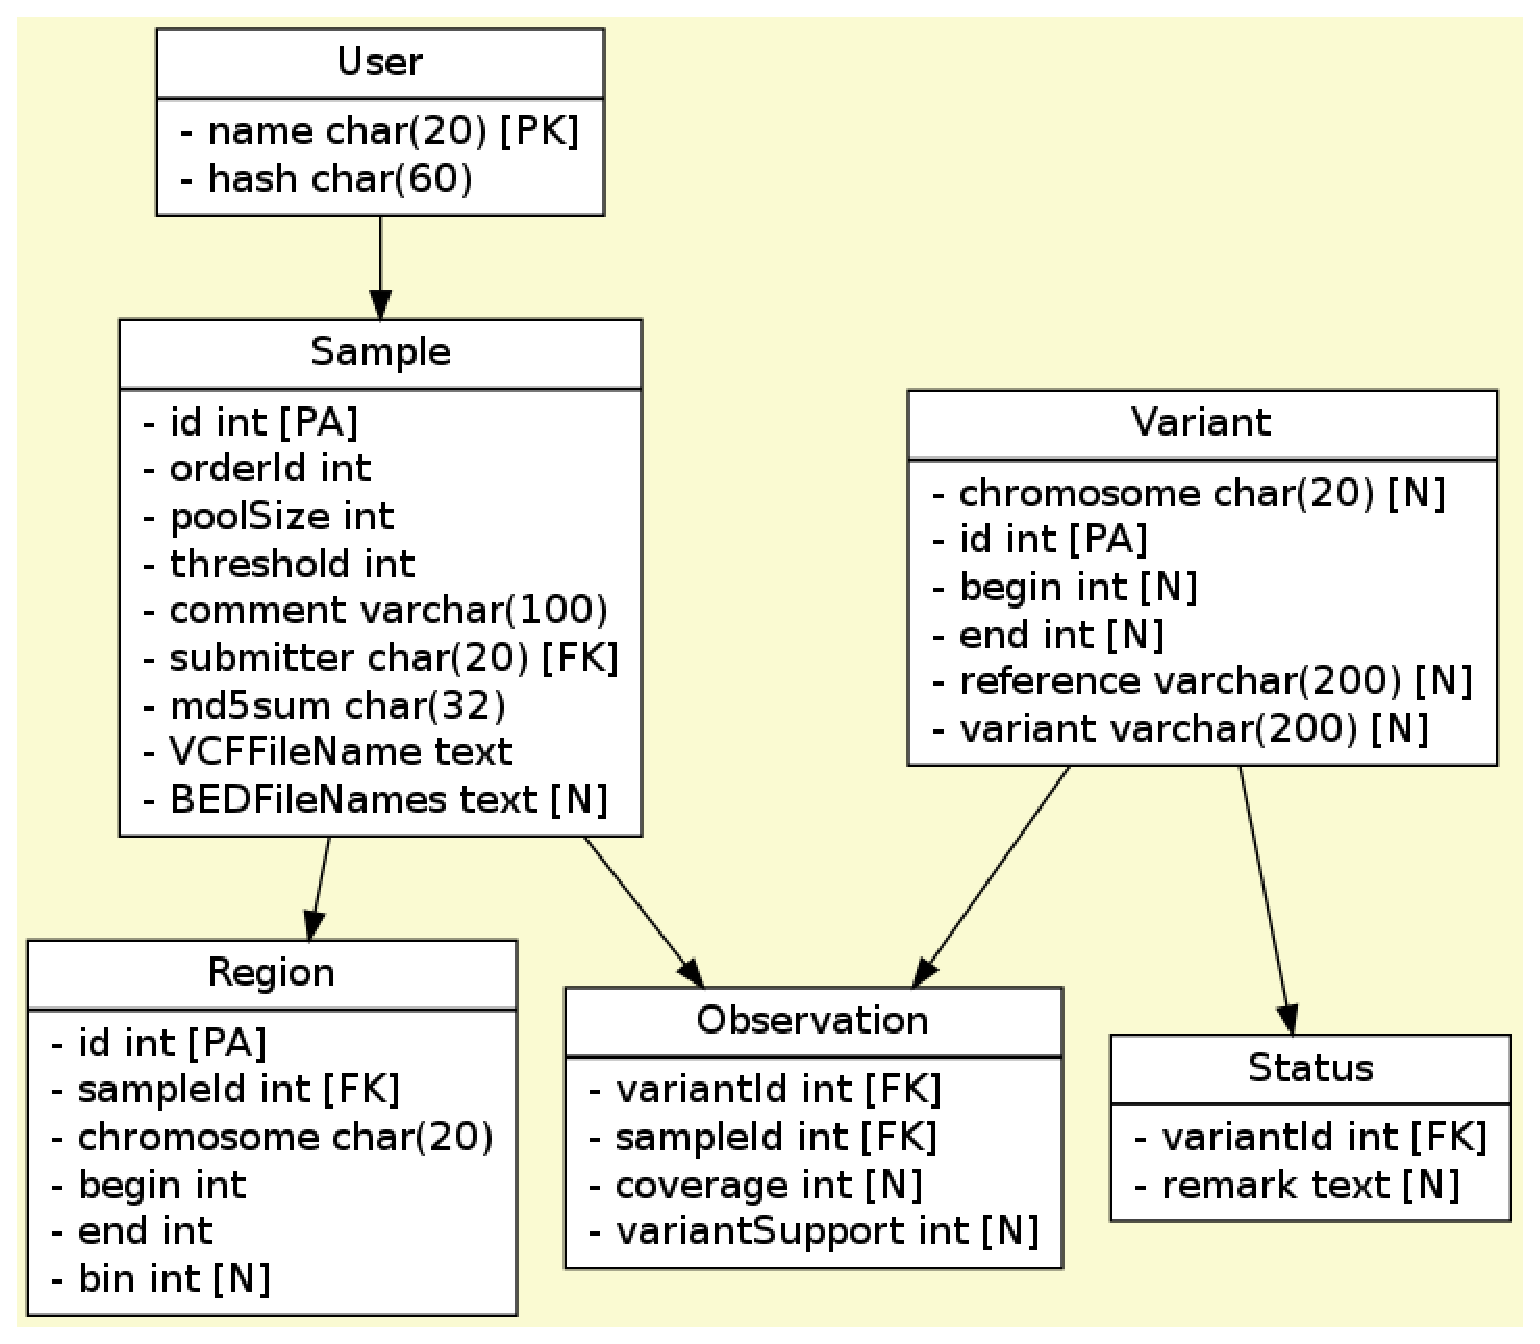
\includegraphics[width=0.8\textwidth]{schema}
  \end{center}
\end{frame}

\section{Using is sharing}

\begin{frame}
  \frametitle{Sample import {\em and} annotation}
  \begin{enumerate}
    \item<1-> Send to the server:
      \begin{itemize}
        \item List of variant (VCF file)
        \item List of covered regions (BED file)
      \end{itemize}
    \item<5-> {\bf Server calculates sample checksum H}
    \item<2-> Server annotates variants with frequencies \uncover<6->{\bf skipping H}
    \item<3-> Download annotation from server
    \item<4-> Server imports variants \uncover<7->{\bf if H is new}
  \end{enumerate}
\end{frame}

\section{Efficient querying}

\begin{frame}
  \frametitle{How indices work}
  Consider a table with 3 columns:
  \begin{itemize}
    \item first name
    \item last name
    \item phone number
  \end{itemize}
  \vspace{0.5cm}
  \pause
  Search on any of the columns, efficiently
  \pause
  \begin{itemize}[<+->]
    \item Solution 1: sort the table
    \item Solution 2: have a separate sorted list of some column(s) with pointers to the table
    \item This is an index
    \item Usually implemented as B-trees
  \end{itemize}
\end{frame}

\begin{frame}
  \frametitle{When indices don't work}
  Consider a table with 2 columns:
  \begin{itemize}
    \item start position
    \item end position
  \end{itemize}
  \vspace{0.5cm}
  \pause
  Search for regions covering some position P, efficiently
  \pause
  \begin{itemize}[<+->]
    \item First find regions with start position smaller than P
    \item In this set, find regions with with end position greater than P
    \item The second part is hard
    \item Simple indices won't help
  \end{itemize}
\end{frame}

\begin{frame}
  \frametitle{Spatial search}
  Searching for regions covering some position is an example of a spatial search
  \begin{itemize}[<+->]
    \item Or: what restaurants are nearby?
    \item Solution: UCSC binning scheme
    \item Essentially the same as R-trees
  \end{itemize}
\end{frame}

\begin{frame}
  \frametitle{UCSC binning scheme: setup}
  Divide genome into bins where for any two, either:
  \begin{enumerate}
    \item one is contained in the other, or
    \item they are non-overlapping
  \end{enumerate}
  \vspace{0.5cm}
  A region gets assigned the smallest bin in which it fits
  \vspace{0.5cm}
  \begin{center}
    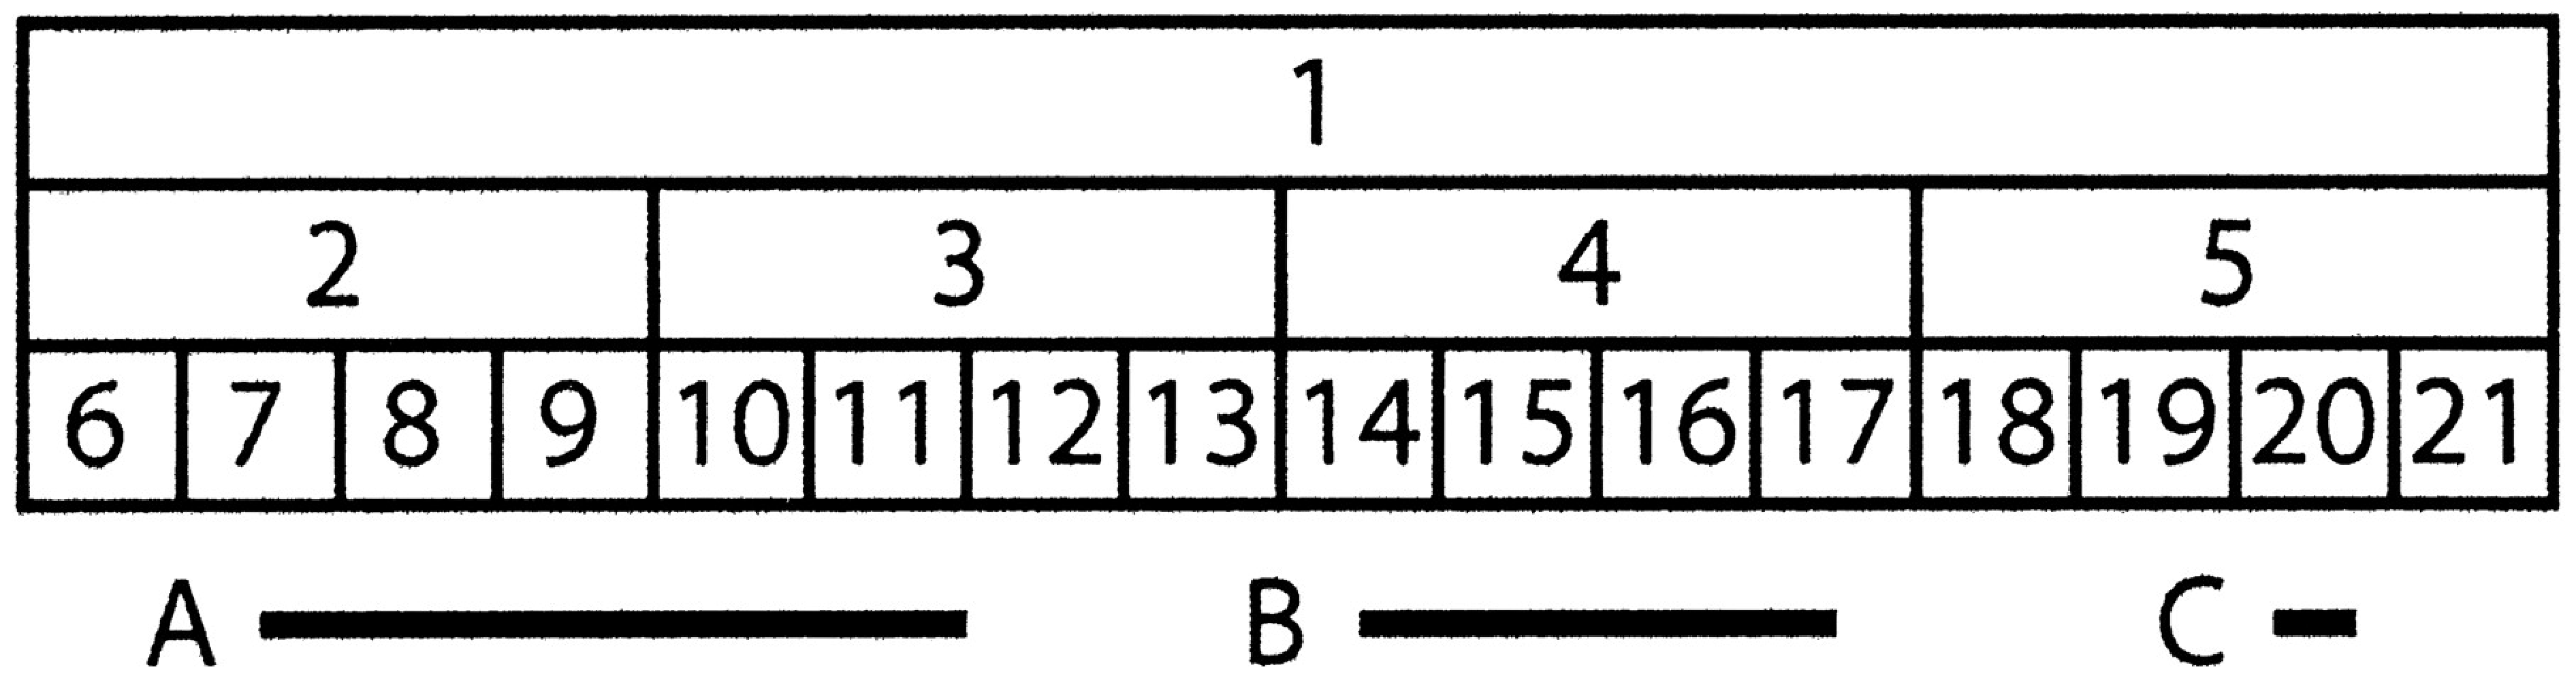
\includegraphics[width=\textwidth]{binning}
  \end{center}
\end{frame}

\begin{frame}
  \frametitle{UCSC binning scheme: spatial search}
  Consider a table with 3 columns:
  \begin{itemize}
    \item start position
    \item end position
    \item bin
  \end{itemize}
  \vspace{0.5cm}
  \pause
  Search for regions covering some position P, efficiently
  \pause
  \begin{itemize}[<+->]
    \item Calculate bins overlapping P
    \item Find regions in these bins
    \item In this set, filter on start and end positions
  \end{itemize}
\end{frame}

\begin{frame}
  \frametitle{Think about your indices}
  Only works with index: (bin, chromosome, start position)\\
  \pause
  \vspace{1cm}
  Time to annotate a sample:
  \begin{itemize}[<+->]
    \item Without index: 4 to 5 hours (and increasing)
    \item With index: 5 to 7 minutes
    \item With index in memory: 30 seconds
  \end{itemize}
\end{frame}

\section{Questions?}
\lastpagetemplate
\begin{frame}
  \begin{center}
    Acknowledgements:\\
    \vspace{0.8cm}
    Jeroen Laros\\
    Bradley ten Broeke\\
    Michiel van Galen\\
    Johan den Dunnen\\
    \vspace{0.8cm}
    Leon Mei (NBIC)\\
    David van Enckevort (NBIC)\\
    The rest of the DVD team
  \end{center}
  \vspace{1cm}
  {\tiny
    \begin{enumerate}
      \item Kent et al. The Human Genome Browser at UCSC. Genome Research 2002.12:996-1006
      \item PyVCF: \texttt{github.com/jamescasbon/PyVCF}
      \item DVD: \texttt{trac.nbic.nl/dvd}
    \end{enumerate}
  }
\end{frame}

\section{Extra}
\extrapagetemplate
\begin{frame}
  \frametitle{Spatial search}
  Alternative solutions?
  \begin{itemize}
    \item Assume regions are of limited length
    \item Assume regions are non-overlapping
    \item 2-column table: position, coverage
    \item Split table on chromosome
    \item Spatial database
  \end{itemize}
  \vspace{1cm}
  All have their downsides
\end{frame}

\end{document}
